\problemname{Cirkelskivevärlden}
It is morning on Discworld, and the sun is about to rise.
The sunrise on Discworld is not like sunrises on most worlds.
This is perhaps not so strange, as Discworld is not like most worlds (it is a disc, as opposed to the more conventional spherical worlds).
Discworld is filled with magic, and as everyone knows, sunlight prefers not to travel through strong magical fields.

As one of Discworld's most powerful wizards living on the opposite side of Discworld from where the sunrise first hits the disc surface, this is a fact you find extremely pleasant.
You love sleeping in, and if you had your way, the sun would preferably stay on its side of the world \emph{some} more hours in the mornings.
Especially now that you have just bought extremely sunlight-sensitive hyacinths.
The silver lining, however, is that as a wizard you can affect the sunlight's advance across Discworld by strengthening certain magical fields in the world.

The world can be modeled as an $n \times n$ grid, where all cells that are part of a disc around the center of the grid exist on the world (exactly which cells exist is given by the input).
In the cell at coordinate $(r, c)$ there is a magical field with strength $m_{r, c}$.
To increase the field strength by $1$, you need to use $p_{r, c}$ spells on the cell.
You cannot increase the field strength by less than $1$, but you can increase it by $1$ repeatedly.

When the sun rises, it starts trying to illuminate position $(0, \frac{n - 1}{2})$ -- at the top of the grid -- and then spreads as follows (see also the figure below).
Suppose the sun tries to illuminate a certain cell $(r, c)$.
It then takes $m_{r, c}$ seconds before the sun shines on the cell.
As soon as the sun shines on the cell, it starts trying to shine on the (up to four) cells that share an edge with it.

You live in cell $(n-1, \frac{n-1}{2})$ (at the bottom of the grid).
In total, you know $k$ spells, which you want to use to increase the field strength in different cells in the world.
Your task is to use the spells in a way that maximizes the number of seconds before the sun illuminates the cell you live in.

\section*{Input}
\textbf{Note:} the test data for this problem is \emph{open}. You can download it in the menu to the right (\texttt{1.in, 2.in, 3.in, 4.in, 5.in}).

The first line contains an integer $0 \le t \le 5$, the ordinal of this test case.
The case $t = 0$ represents the sample case, and should be ignored (you can print anything).

The second line contains two integers $n$ and $k$, where $n$ is odd.

The following $n$ lines contain the values $m_{r, c}$.
The $i$th line contains the values $m_{i, c}$ for all $0 \le c < n$.

The following $n$ lines contain the values $p_{r, c}$.
The $i$th line contains the values $p_{i, c}$ for all $0 \le c < n$.

If a cell is not on the disc, both $m_{r, c}$ and $p_{r, c}$ are $-1$; otherwise they are always positive.

\section*{Output}
Print $n$ lines with $n$ numbers each.
The $i$th line should contain the number of spells you use on cells $(i, c)$ for $0 \le c < n$.
The number of spells you use on cell $(i, c)$ must be a multiple of $p_{i, c}$.

\section*{Scoring}
Your solution will receive points on each of the five test cases.

Each test case is scored as follows.
Suppose the time it takes for the sun to reach you is $T$ seconds if no spells are used, that the maximum time any participant achieves is $T_{max}$, and that your time is $T_{you}$.

Your score on the test case is then

\[ 20 \cdot \frac{T_{you} - T}{T_{max} - T}. \]

During the competition, $T_{max}$ will be set to $2 \cdot T$.

\section*{Explanation of the sample}
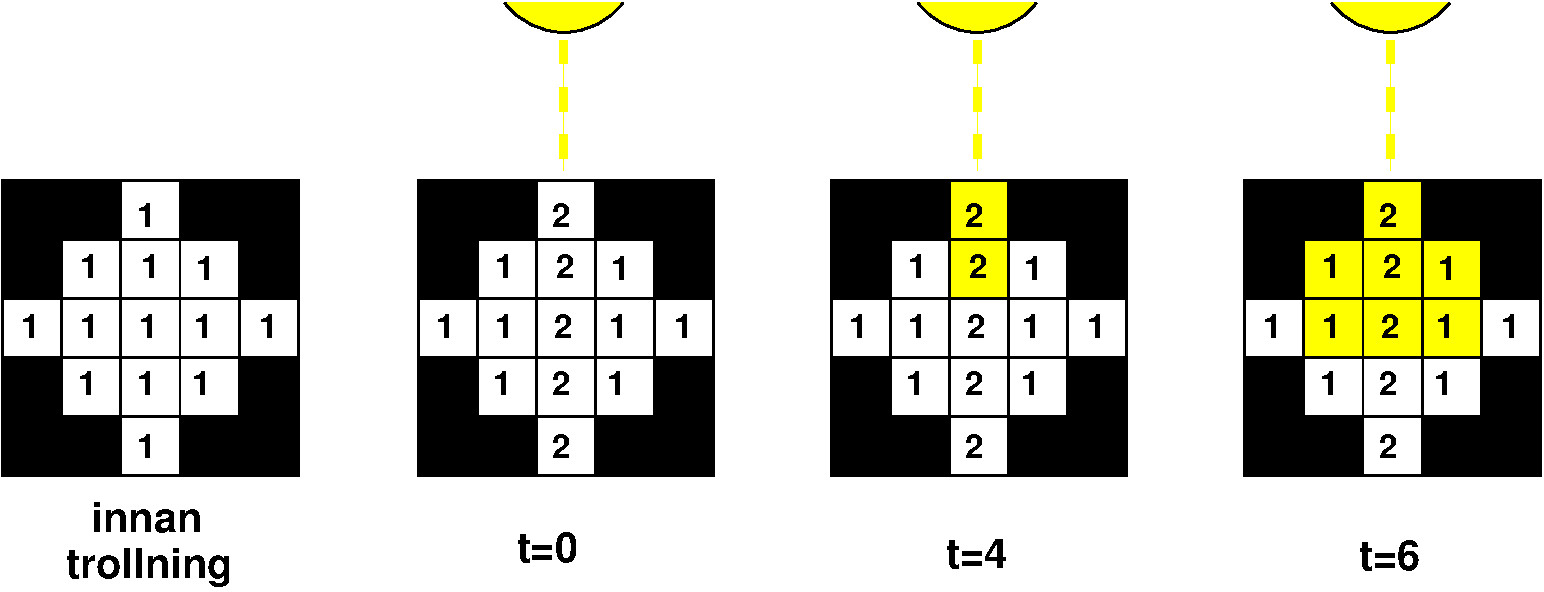
\includegraphics[width=14cm]{disc.pdf}\\
{\em The numbers indicate the magical field strength before casting (left figure) and after casting (remaining figures). The color marking shows which cells are illuminated after 0, 4, and 6 seconds respectively. The bottom cell, where you live, becomes illuminated after 10 seconds. There are many other ways of casting that give the same delay.}
